% !TEX root = ../main.tex
\begin{frame}\begin{center}
\LARGE\textbf{Example}
\end{center}\end{frame}
%-------------------------------------------------------------------------------
%-------------------------------------------------------------------------------
\begin{frame}\textbf{Seminal paper}\vspace{0.3cm}
\begin{itemize}
\item \bibentry{Keane.1997}
\end{itemize}
\end{frame}
%-------------------------------------------------------------------------------
%-------------------------------------------------------------------------------
\begin{frame}\textbf{Model of occupational choice}\vspace{0.3cm}

\begin{itemize}\setlength\itemsep{1em}
\item life cycle histories \medskip
\begin{itemize}\setlength\itemsep{1em}
\item school attendance
\item occupation-specific work status
\item wages
\end{itemize}
\end{itemize}
\end{frame}

%-------------------------------------------------------------------------------
%-------------------------------------------------------------------------------
\begin{frame}
\begin{figure}
  \caption{Decision tree}
  \scalebox{0.70}{% Decision tree

\tikzset{
	treenode/.style = {shape=rectangle, rounded corners, draw, align=center, bottom color=blue!20},
	root/.style     = {treenode, font=\small, draw=none},
	env/.style      = {treenode, font=\small, draw=none},
	dummy/.style    = {circle,draw}
}


\begin{tikzpicture}
[
	x=30pt,
	y=26pt,
	yscale=-1,
	xscale=1,
	baseline=-120pt,
	grow                    = right,
	edge from parent/.style = {draw, -latex},
	every node/.style       = {font=\footnotesize, minimum width={width("Magnetometer")+2pt}},
	sloped
]


% Zero  level: START
\node [root, top color = tabgrey, bottom color = tabgrey] (0) at (-10,0) {\textbf{Start}};


% First level: HOME
\node [env, top color = tabgreen, bottom color = tabgreen, scale = 0.8] (1) at (-5,-4.2) {\textbf{Home}};
\draw[->, thick] (0) edge node[left of = 0, rotate = 72.75, node distance = 0.3cm]{$10.56\,\%$} (1);
% Second level: Home, School, Blue, White, Military
\node [env, top color = tabgreen, bottom color = tabgreen, scale = 0.55] (11) at (0,-5) {Home};
\draw[->] (1) edge (11);
\node [env, top color = taborange, bottom color = taborange, scale = 0.55] (12) at (0,-4.6) {School};
\draw[->] (1) edge (12);
\node [env, top color = tabblue, bottom color = tabblue, scale = 0.55] (13) at (0,-4.2) {Blue};
\draw[->] (1) edge (13);
\node [env, top color = tabred, bottom color = tabred, scale = 0.55] (14)  at (0,-3.8) {White};
\draw[->] (1) edge (14);
\node [env, top color = tabpurple, bottom color = tabpurple, scale = 0.55] (15)  at (0,-3.4) {Military};
\draw[->] (1) edge (15);
% Third level coordinates
\coordinate (a1) at (3,-5);
\draw [->, dashed, color = tabgrey] (11) to[right] node[auto] {} (a1);
\coordinate (a2) at (3,-4.6);
\draw [->, dashed, color = tabgrey] (12) to[right] node[auto] {} (a2);
\coordinate (a3) at (3,-4.2);
\draw [->, dashed, color = tabgrey] (13) to[right] node[auto] {} (a3);
\coordinate (a4) at (3,-3.8);
\draw [->, dashed, color = tabgrey] (14) to[right] node[auto] {} (a4);
\coordinate (a5) at (3,-3.4);
\draw [->, dashed, color = tabgrey] (15) to[right] node[auto] {} (a5);



%First level: School
\node [env, top color = taborange, bottom color = taborange, scale = 0.8] (2) at (-5,-2.1) {\textbf{School}};
\draw[->, thick] (0) edge node[right of = 0, yshift = 0.35cm,  rotate = 41.0, node distance = 0cm]{$85.80\,\%$} (2);
% Second level: Home, School, Blue, White, Military
\node [env, top color = tabgreen, bottom color = tabgreen, scale = 0.55] (21) at (0,-2.9) {Home};
\draw[->] (2) edge (21);
\node [env, top color = taborange, bottom color = taborange, scale = 0.55] (22) at (0,-2.5) {School};
\draw[->] (2) edge (22);
\node [env, top color = tabblue, bottom color = tabblue, scale = 0.55] (23) at (0,-2.1) {Blue};
\draw[->] (2) edge (23);
\node [env, top color = tabred, bottom color = tabred, scale = 0.55] (24)  at (0,-1.7) {White};
\draw[->] (2) edge (24);
\node [env, top color = tabpurple, bottom color = tabpurple, scale = 0.55] (25)  at (0,-1.3) {Military};
\draw[->] (2) edge (25);
% Second level --> third level
\coordinate (e1) at (3,-2.9);
\draw [->, dashed, color = tabgrey] (21) to[right] node[auto] {} (e1);
\coordinate (e2) at (3,-2.5);
\draw [->, dashed, color = tabgrey] (22) to[right] node[auto] {} (e2);
\coordinate (e3) at (3,-2.1);
\draw [->, dashed, color = tabgrey] (23) to[right] node[auto] {} (e3);
\coordinate (e4) at (3,-1.7);
\draw [->, dashed, color = tabgrey] (24) to[right] node[auto] {} (e4);
\coordinate (e5) at (3,-1.3);
\draw [->, dashed, color = tabgrey] (25) to[right] node[auto] {} (e5);


% First Level: Blue
\node [env, top color = tabblue, bottom color = tabblue, scale = 0.8] (3) at (-5,0) {\textbf{Blue}};
\draw[->, thick] (0) edge node[right of = 0, yshift = 0.25cm, node distance = 0.2cm]{$3.28\,\%$} (3);
% Second level: Home, School, Blue, White, Military
\node [env, top color = tabgreen, bottom color = tabgreen, scale=0.55] (31) at (0,-0.8) {Home};
\draw[->] (3) edge (31);
\node [env, top color = taborange, bottom color=taborange, scale = 0.55] (32) at (0,-0.4) {School};
\draw[->] (3) edge (32);
\node [env, top color = tabblue, bottom color = tabblue, scale = 0.55] (33) at (0,0) {Blue};
\draw[->] (3) edge (33);
\node [env, top color = tabred, bottom color = tabred, scale = 0.55] (34)  at (0,0.4) {White};
\draw[->] (3) edge (34);
\node [env, top color = tabpurple, bottom color = tabpurple, scale = 0.55] (35)  at (0,0.8) {Military};
\draw[->] (3) edge (35);
% Second level --> third level
\coordinate (c1) at (3,-0.8);
\draw [->, dashed, color = tabgrey] (31) to[right] node[auto] {} (c1);
\coordinate (c2) at (3,-0.4);
\draw [->, dashed, color = tabgrey] (32) to[right] node[auto] {} (c2);
\coordinate (c3) at (3,0);
\draw [->, dashed, color = tabgrey] (33) to[right] node[auto] {} (c3);
\coordinate (c4) at (3,0.4);
\draw [->, dashed, color = tabgrey] (34) to[right] node[auto] {} (c4);
\coordinate (c5) at (3,0.8);
\draw [->, dashed, color = tabgrey] (35) to[right] node[auto] {} (c5);


% First Level: White
\node [env, top color = tabred, bottom color = tabred, scale = 0.8] (4)  at (-5,2.1) {\textbf{White}};
\draw[->, thick] (0) edge node[right of = 0, yshift = 0.1cm, rotate = -38, node distance = 0.25cm]{$0.29\,\%$} (4);
% Second level: Home, School, Blue, White, Military
\node [env, top color = tabgreen, bottom color = tabgreen, scale = 0.55] (41) at (0,1.3) {Home};
\draw[->] (4) edge (41);
\node [env, top color = taborange, bottom color = taborange, scale = 0.55] (42) at (0,1.7) {School};
\draw[->] (4) edge (42);
\node [env, top color = tabblue, bottom color = tabblue, scale = 0.55] (43) at (0,2.1) {Blue};
\draw[->] (4) edge (43);
\node [env, top color = tabred, bottom color = tabred, scale = 0.55] (44)  at (0,2.5) {White};
\draw[->] (4) edge (44);
\node [env, top color = tabpurple, bottom color = tabpurple, scale = 0.55] (45)  at (0,2.9) {Military};
\draw[->] (4) edge (45);
% Second level --> third level
\coordinate (b1) at (3,1.3);
\draw [->, dashed, color = tabgrey] (41) to[right] node[auto] {} (b1);
\coordinate (b2) at (3,1.7);
\draw [->, dashed, color = tabgrey] (42) to[right] node[auto] {} (b2);
\coordinate (b3) at (3,2.1);
\draw [->, dashed, color = tabgrey] (43) to[right] node[auto] {} (b3);
\coordinate (b4) at (3,2.5);
\draw [->, dashed, color = tabgrey] (44) to[right] node[auto] {} (b4);
\coordinate (b5) at (3,2.9);
\draw [->, dashed, color = tabgrey] (45) to[right] node[auto] {} (b5);


% First Level: Military
\node [env, top color = tabpurple, bottom color = tabpurple, scale = 0.8] (5)  at (-5,4.2) {\textbf{Military}};
\draw[->, thick] (0) edge node[right of = 0, yshift=0.25cm, rotate = -72.75, node distance = 0.15cm]{$0.07\,\%$} (5);
%\draw[->, thick] (0) edge (5);
% Second level: Home, School, Blue, White, Military
\node [env, top color = tabgreen, bottom color = tabgreen, scale = 0.55] (51)  at (0,3.4) {Home};
\draw[->] (5) edge (51);
\node [env, top color = taborange, bottom color = taborange, scale = 0.55] (52)  at (0,3.8) {School};
\draw[->] (5) edge (52);
\node [env, top color = tabblue, bottom color = tabblue, scale = 0.55] (53) at (0,4.2) {Blue};
\draw[->] (5) edge (53);
\node [env, top color = tabred, bottom color = tabred, scale = 0.55] (54) at (0,4.6) {White};
\draw[->] (5) edge (54);
\node [env, top color = tabpurple, bottom color = tabpurple, scale = 0.55] (55) at (0,5.0) {Military};
\draw[->] (5) edge (55);
% Second level --> third level
\coordinate (d1) at (3,3.4);
\draw [->, dashed, color = tabgrey] (51) to[right] node[auto] {} (d1);
\coordinate (d2) at (3,3.8);
\draw [->, dashed, color = tabgrey] (52) to[right] node[auto] {} (d2);
\coordinate (d3) at (3,4.2);
\draw [->, dashed, color = tabgrey] (53) to[right] node[auto] {} (d3);
\coordinate (d4) at (3,4.6);
\draw [->, dashed, color = tabgrey] (54) to[right] node[auto] {} (d4);
\coordinate (d5) at (3,5.0);
\draw [->, dashed, color = tabgrey] (55) to[right] node[auto] {} (d5);

\end{tikzpicture}

\vspace{1cm}}
\end{figure}
\end{frame}
%-------------------------------------------------------------------------------
%-------------------------------------------------------------------------------
\begin{frame}\textbf{Immediate utility}\vspace{0.3cm}

  \begin{align*}
  u(\cdot) =
  \begin{cases}
      \zeta_a(\cdot)  + w_a(\cdot)                & \text{if}\, a \in \{1, 2, 3\}  \\
      \zeta_a(\cdot)                                                  &  \text{if}\, a \in \{4, 5\}
  \end{cases}
  \end{align*}

\begin{table}[]
	\hskip1.5cm
	\begin{tabular}{ll}
	$\zeta_a(\cdot)$	& non-pecuniary utility \\[-0.5em]
	$w_a(\cdot) $	& wage component
	\end{tabular}
\end{table}

\end{frame}
%-------------------------------------------------------------------------------
%-------------------------------------------------------------------------------
\begin{frame}\textbf{Transitions}\vspace{0.3cm}

  Work experience $\bm{k_t}$  and years of completed schooling $h_t$ evolve deterministically.

  \begin{align*}
  k_{a,t+1} = k_{a,t} + \ind[a_t = a]  &\qquad \text{if}\, a \in \{1, 2, 3\} \\
  h_{t + 1\phantom{,a}} = h_{t\phantom{,a}} +   \ind[a_t = 4]  &\qquad\\
  \end{align*}

  Productivity shocks $\bm{e_t}$ are uncorrelated across time and follow a multivariate normal distribution with mean $\bm{0}$ and covariance matrix $\bm{\Sigma}$.

\end{frame}
%-------------------------------------------------------------------------------
%-------------------------------------------------------------------------------
\begin{frame}\textbf{Non-pecuniary utility of blue-collar occupation}\vspace{0.3cm}
%
  \begin{align*}
  \zeta_{1}(\cdot)  = \alpha_1 & + c_{1,1} \cdot \ind[a_{t-1} \neq 1] + c_{1,2} \cdot \ind[k_{1,t} = 0] \\
                              & + \vartheta_1 \cdot \ind[h_t \geq 12] + \vartheta_2 \cdot \ind[h_t \geq 16] + \vartheta_3 \cdot \ind[k_{3,t} = 1]
  \end{align*}
\end{frame}
%-------------------------------------------------------------------------------
%-------------------------------------------------------------------------------
\begin{frame}\textbf{Wage component}\vspace{0.3cm}
%
\begin{align*}
w_{a}(\cdot) & = r_{a} \, x_{a}(\cdot)
\end{align*}

with skill production function

\begin{align*}
x_{1}(\cdot) & = \exp \big( \Gamma_{1}(\bm{k_t},  h_t, t, a_{t-1}, e_{j,1}) \cdot \epsilon_{1,t} \big).
\end{align*}
\end{frame}
%-------------------------------------------------------------------------------
%-------------------------------------------------------------------------------
\begin{frame}\textbf{Skill production for blue-collar occupation}\vspace{0.3cm}
%
\begin{align*}
     \Gamma_1(\cdot) = e_{j,1} & + \beta_{1,1} \cdot h_t + \beta_{1, 2} \cdot \ind[h_t \geq 12] + \beta_{1,3} \cdot \ind[h_t\geq 16]\\
                                   & + \gamma_{1, 1} \cdot  k_{1,t} + \gamma_{1,2} \cdot  (k_{1,t})^2 + \gamma_{1,3} \cdot  \ind[k_{1,t} > 0] \\
                                 & + \gamma_{1,4} \cdot  t + \gamma_{1,5} \cdot \ind[t < 18]\\
                                   & + \gamma_{1,6} \cdot \ind[a_{t-1} = 1] + \gamma_{1,7} \cdot  k_{2,t} + \gamma_{1,8} \cdot  k_{3,t}
\end{align*}
%
\end{frame}
%-------------------------------------------------------------------------------
%-------------------------------------------------------------------------------
\begin{frame}\begin{center}
		\LARGE\textit{Empirical data}
\end{center}\end{frame}
%-------------------------------------------------------------------------------
%-------------------------------------------------------------------------------
\begin{frame}\textbf{National Longitudinal Survey of Youth 1979}\vspace{0.3cm}

\begin{itemize}\setlength\itemsep{1em}
\item 1,373 individuals starting at age 16
\item life cycle histories \medskip
\begin{itemize}\setlength\itemsep{1em}
\item school attendance
\item occupation-specific work status
\item wages
\end{itemize}
\end{itemize}
\end{frame}
%-------------------------------------------------------------------------------
%-------------------------------------------------------------------------------
\begin{frame}
  \begin{figure}
  \caption{Choices}
  \scalebox{0.35}{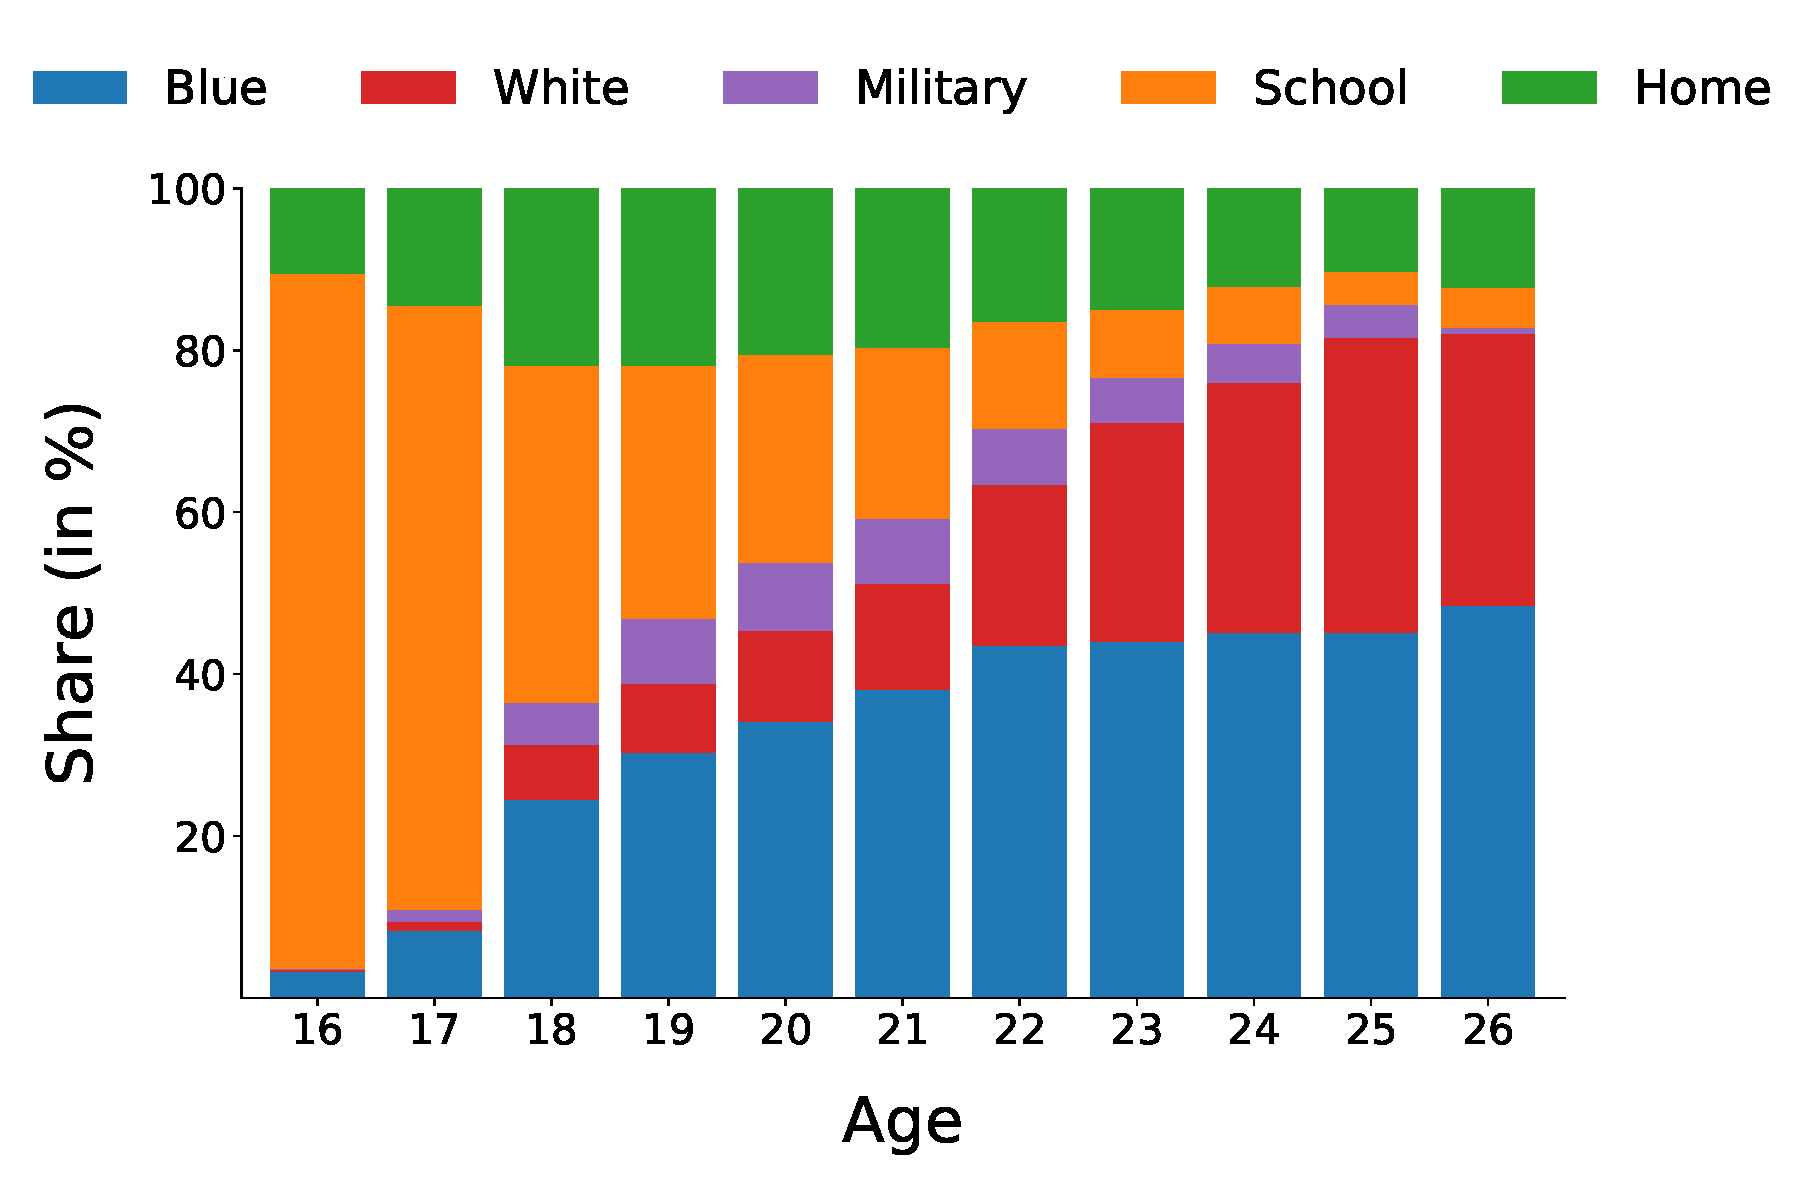
\includegraphics{fig-data-choice-all}}
  \end{figure}
\end{frame}

%-------------------------------------------------------------------------------
%-------------------------------------------------------------------------------
\begin{frame}
  \begin{figure}
  \caption{Average wage}
  \scalebox{0.35}{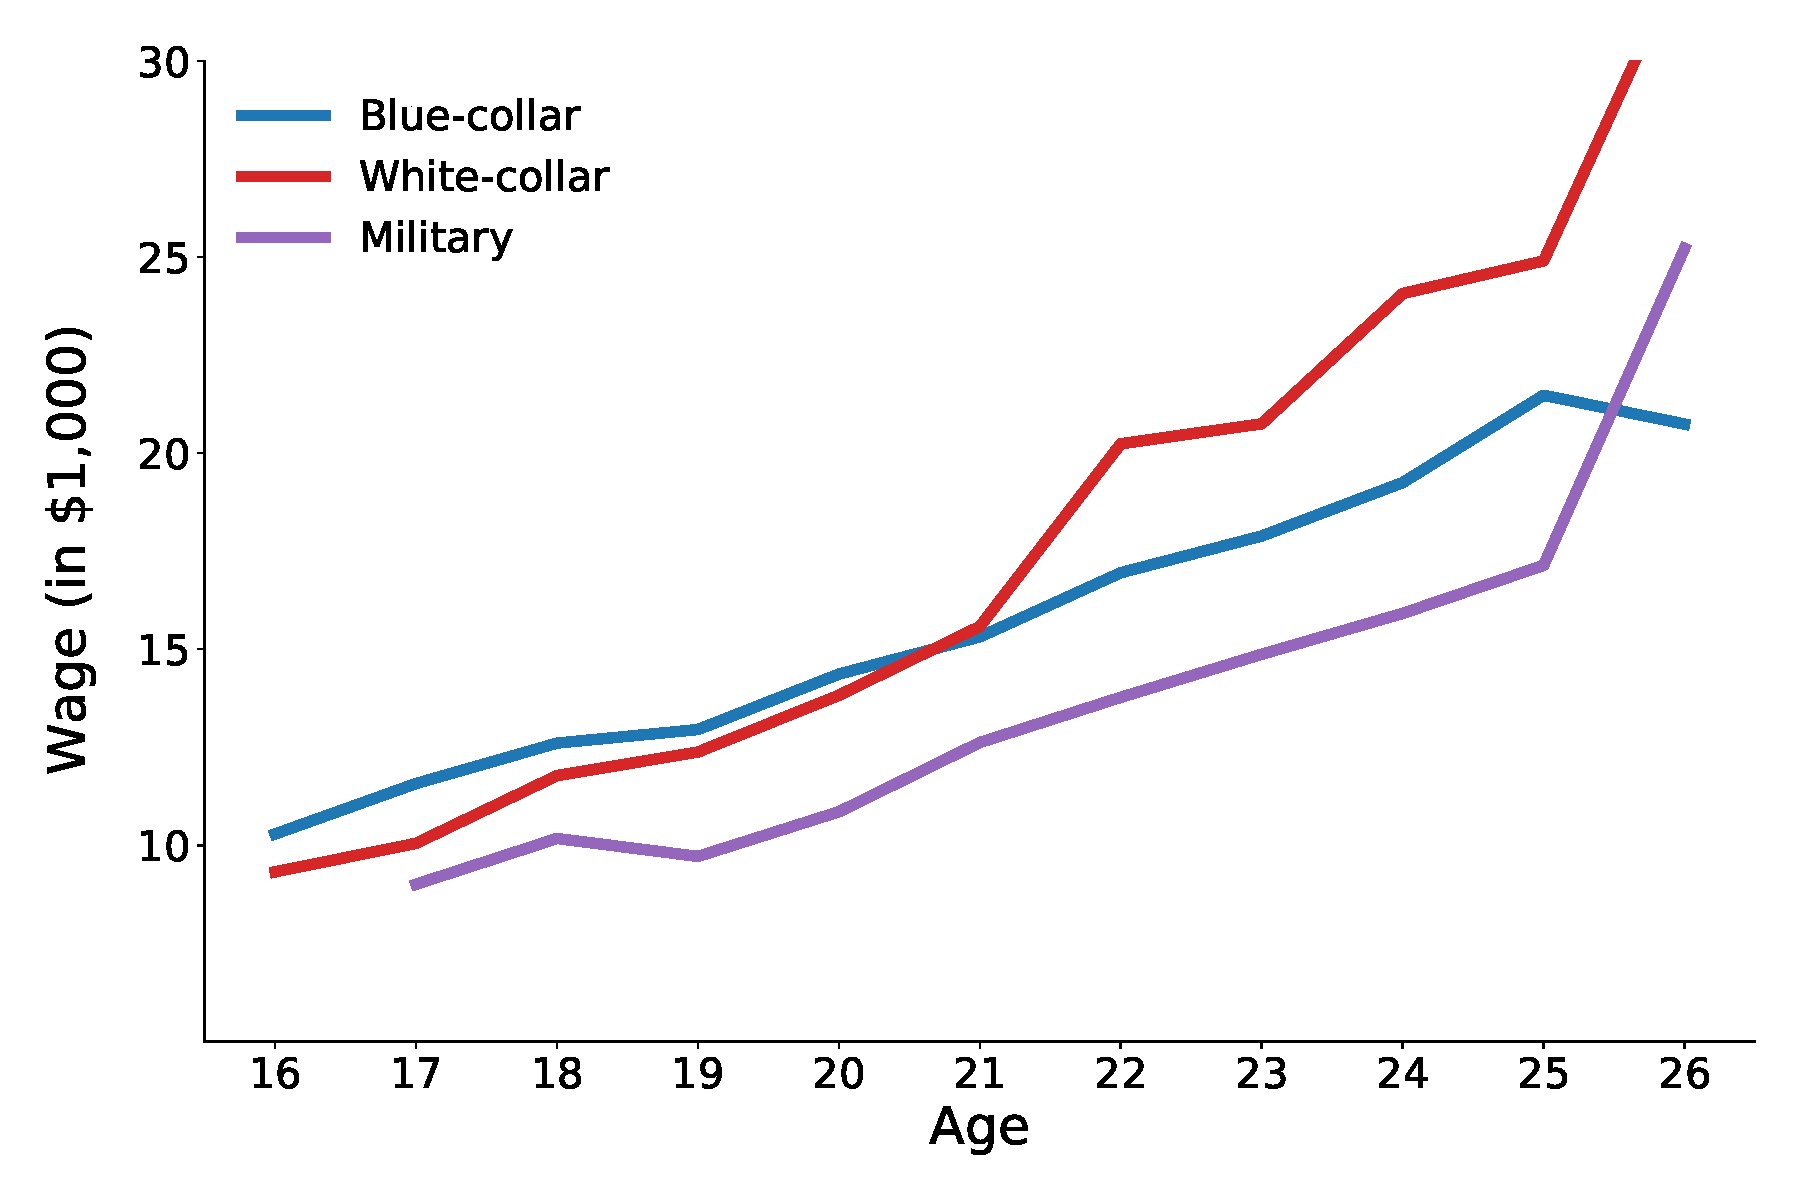
\includegraphics{fig-data-wage-occupations}}
  \end{figure}
\end{frame}
%-------------------------------------------------------------------------------
%-------------------------------------------------------------------------------
\begin{frame}\begin{center}
		\LARGE\textit{Economic insights}
\end{center}\end{frame}
%-------------------------------------------------------------------------------
%-------------------------------------------------------------------------------
\begin{frame}
  \begin{figure}[h!]\centering
  \caption{Economic mechanism and policy forecast}\label{Economic mechanism and policy forecast}
  \subfloat[Time preference]{\scalebox{0.175}{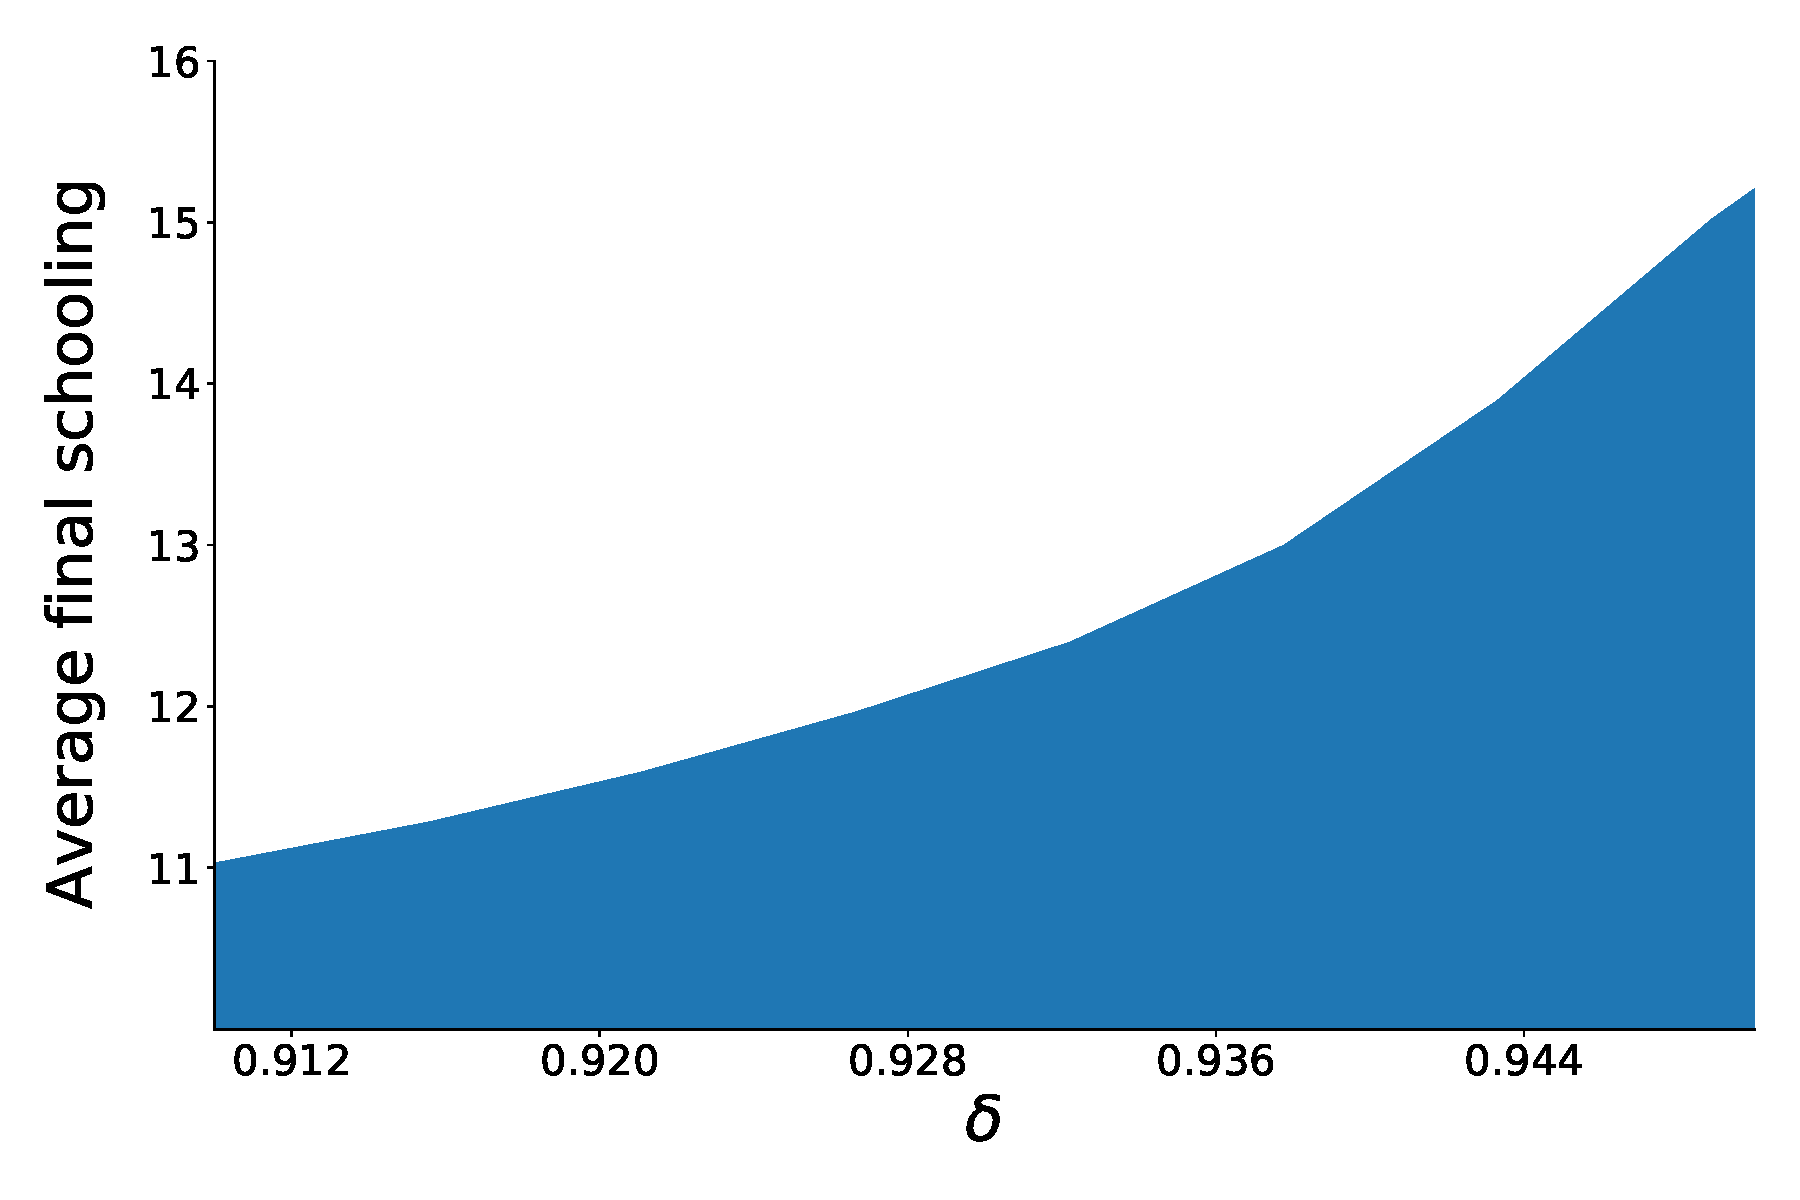
\includegraphics{fig-economic-mechanism}}}\hspace{0.3cm}
  \subfloat[Tuition subsidy]{\scalebox{0.175}{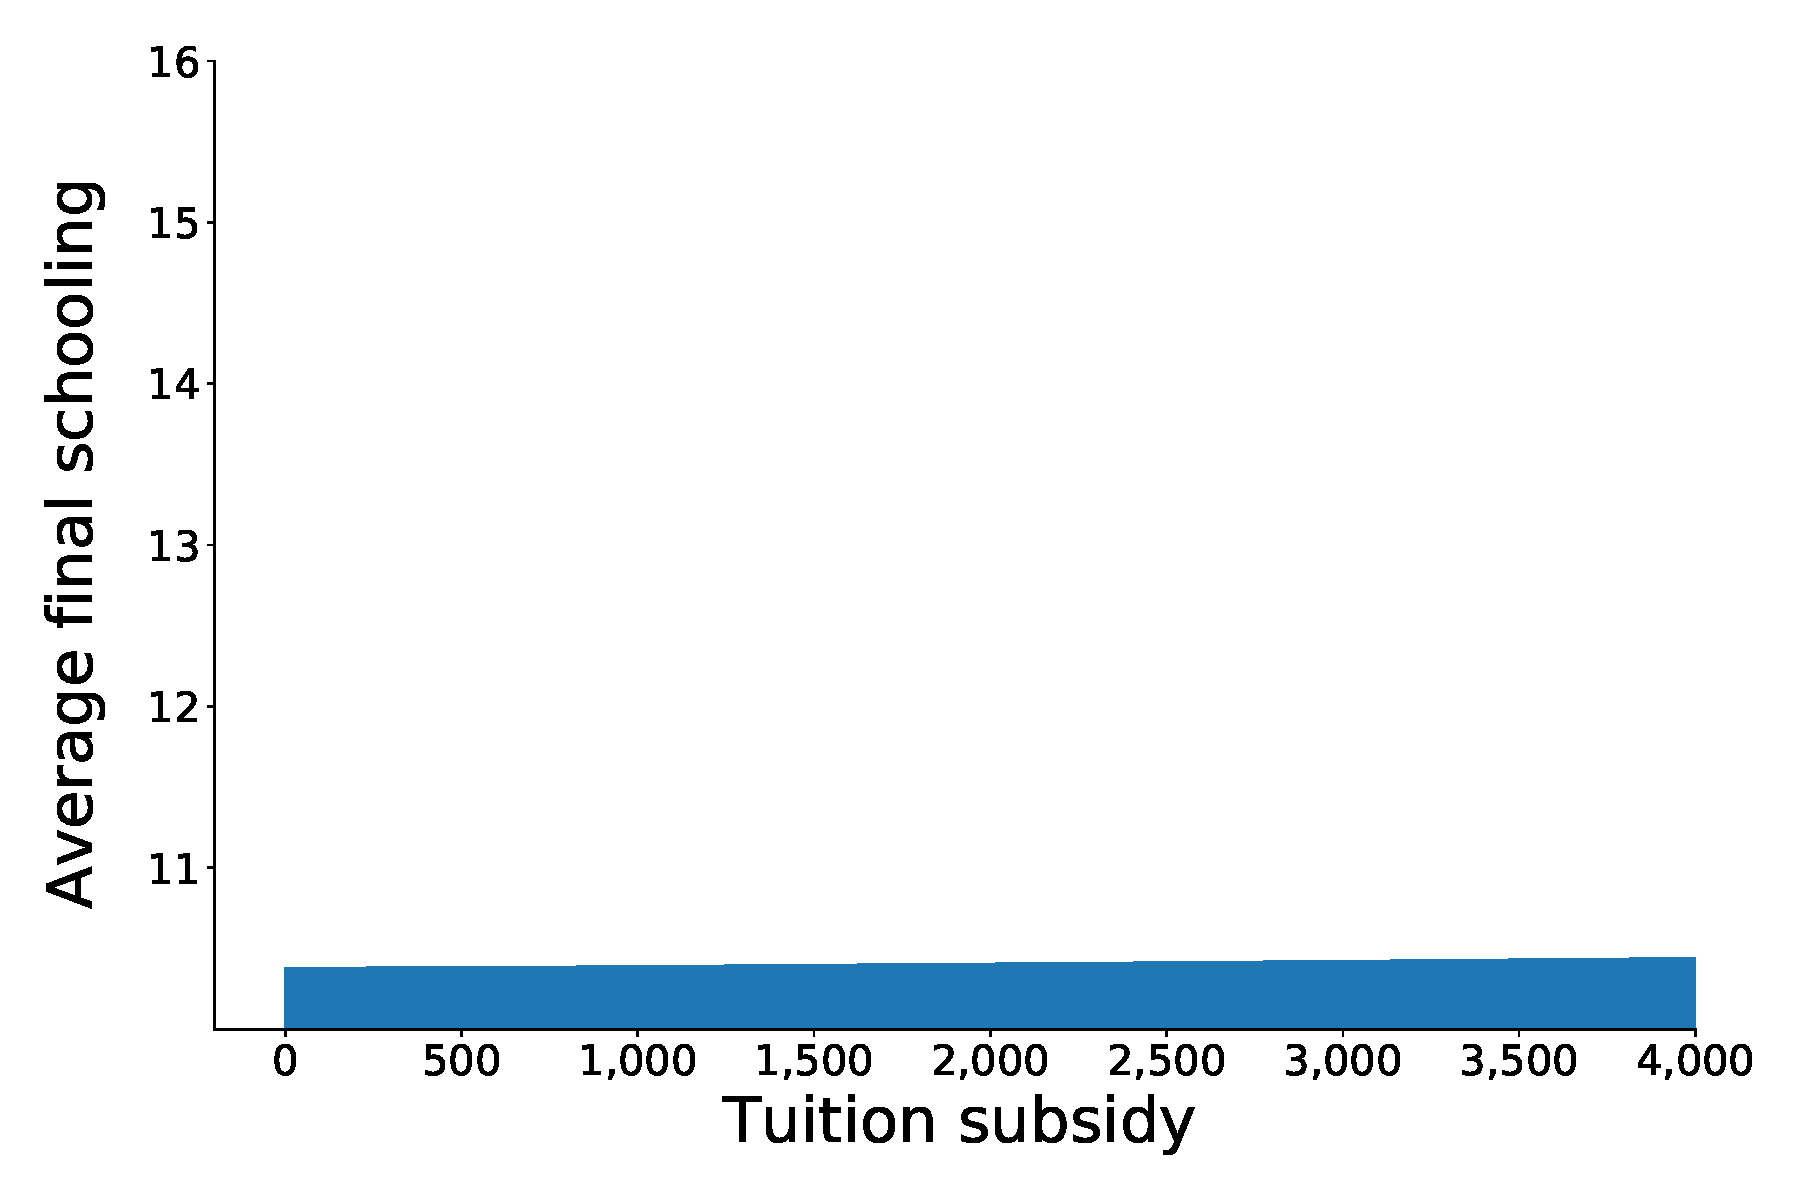
\includegraphics{fig-policy-forecast}}}
  \end{figure}
\end{frame}
